\documentclass[12pt]{article}

\setlength{\topmargin}{-.5in}
\setlength{\textheight}{9in}
\setlength{\oddsidemargin}{.125in}
\setlength{\textwidth}{6.25in}
\usepackage{amsmath}
\usepackage{verbatim}
\usepackage{graphicx}
\newcommand{\TODO}[1]{\textcolor{red}{\textbf{[TODO:#1]}}}
\usepackage{listings}
\usepackage{color}
\usepackage{url}
\usepackage{syntax}
  \usepackage{tabularx}
  \usepackage{graphicx}
\definecolor{gray}{rgb}{0.5,0.5,0.5}
\definecolor{mauve}{rgb}{0.58,0,0.82}
\usepackage{amsmath}
\usepackage{verbatim}
\usepackage{graphicx}
\begin{document}

\begin{titlepage}

\begin{figure}[t]
    \centering
    
\includegraphics[scale=0.4]{./draws/inria-logo.png}
\end{figure}

\vspace*{2cm}
\begin{center}
	{\huge \textbf{VCE v4 Tutorial}} \vspace*{1cm}
\\
    {\large INRIA – Sophia-Antipolis } \medskip \\
\end{center}

%
\vfill
\begin{center}
\begin{minipage}[b]{0.5\textwidth}
    \vspace*{1.3cm}
    \begin{center}
        {\large July 2015}
    \end{center}
        \begin{center}
        {\large oleksandra.kulankhina@inria.fr}
    \end{center}
     \vspace*{1cm}
        \begin{center}
        {\large VCE version 4.0.2}
    \end{center}
\end{minipage}%
\end{center}

\thispagestyle{empty}

\end{titlepage}

\tableofcontents
\newpage

\section{Introduction}\label{sec:intro}
VerCors is a platform for the specification, analysis, verification and validation of the GCM- 
based applications architecture and behavior. It contains a set of tools including VCE v.4. VCE v.4 is a graphical designer for the GCM architecture and the Components behavior specification. It is distributed as a set of Eclipse plugins.

This guide explains the basic functionality of VCE v.4. 
It provides step by step instructions for creating a simple example of a Component model using the VCE editors, including all facets of this model: classes and interfaces, types, architecture, and behaviors. It also explains how to validate the static semantics properties of the Component models, how to produce (partial) executable code in GCM/ProActive and how to produce models that can be verified be CADP\footnote{http://cadp/} model-checker.

\textbf{Additional information:}

VCE v.4 is based on Sirius\footnote{http://www.eclipse.org/sirius/} technology and on the functionality of the standard editors created with Sirius. Hence, if one wants to get more specific/advanced information that would not be found in this tutorial, it is recommended to read some of the Sirius documentations. In particular:
\begin{itemize}
\item
Getting started for End-users: https://wiki.eclipse.org/Sirius/Tutorials/4MinTutorial
\item
Sirius user manual: http://www.eclipse.org/sirius/doc/user/Sirius\%20User\%20Manual.html
\end{itemize}

\subsection{VCEv4 Overview}
As in all Eclipse-based environments, all models and diagrams related to a given application are grouped in a Project. 

A \textbf{VCE Modeling project} contains models (\textbf{VCE} models for the architecture description, \textbf{UML} classes and interfaces, UML State Machines for behavior description, and \textbf{VceTypes} models for types definition). A VCE Modeling project also includes  diagrams (VCE Components diagrams, UML classes, interfaces, and state-machine diagrams and a VCE Types diagram) which illustrate the elements of the models. A VCE model has links to UML models. In particular, a GCM interface refers to a UML Interface, a GCM Primitive component refers to a UML Class. The UML Operations and State Machines use VCE Types for the typing of the arguments and return values. 

VCEv4 mainly contains three modules:
\begin{itemize}
\item
Graphical editors for architecture and behavior design;
\item
A module translating graphical models into Executable Java/Proactive code;
\item
A module translating graphical models into input for CADP model-checker.
\end{itemize}

\subsection{Properties view}

You will often need to edit some parameters of your model in \textbf{Properties} view of Eclipse. If you do not see it in your workspace, in order to open it you should:

\begin{enumerate}
\item
Click on \textbf{Window} on the top-bar menu of Eclipse (Obeo) and select \textbf{Show view $\rightarrow$ Properties}.
\end{enumerate}

\section{Architecture and Behavior graphical specification}\label{sec:graph}
In this section we explain how to:
\begin{itemize}
\item
create a new VCE Project or import it from an existing source;
\item
edit GCM Component diagrams;
specify types;
\item
create and edit UML classes, interfaces, operations and attributes;
\item
connect the operations of UML classes and interfaces;
\item
attach a UML interface to a GCM interface;
\item
attach a UML class to a GCM primitive component;
\item
specify default values of UML attributes;
\item
create and edit a State Machine and attach it to a UML operation.
\end{itemize}

We will illustrate the use of graphical editors with an example described in the section below.

\subsection{Example Overview}

A figure below illustrates the example. This is a very simple VCE Component diagram containing one primitive component \textbf{Prim1} with one server and one client GCM interface (\textbf{S1} and \textbf{C1}). Each GCM interface is connected to a UML interface (\textbf{Interface1} and \textbf{Interface2} respectively). Interface1 has an operation \textbf{sumUp} that can be served by the component, Interface2 has the list of the operations that can be called by the component. A UML class \textbf{Class1} is attached to the component. It has one method implementing the operation of the server interface (\textbf{sumUp()}), one attribute \textbf{last\_sum} and two methods \textbf{get\_last\_sum()} and \textbf{set\_last\_sum()} to access the value of the attribute. The behavior of the sumUp  method is illustrated on a UML State Machine sumUp. The default value of attribute \textbf{last\_sum} is given in a green box and is equal to 0.

%\begin{figure}
     \centerline{
     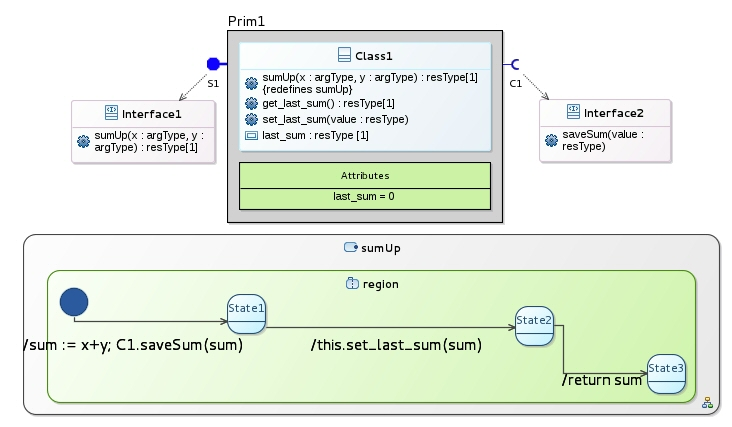
\includegraphics[width=14cm]{draws/example-full.jpg}
  %   \caption{VCE Components diagram}
     \label{fig:example-full}
     }
% \end{figure}

Prim1 implements the following business logic. Method sumUp can be called on the server interface S1. It takes two arguments: x and y, computes their sum, saves the sum to its local attribute last\_sum, sends the sum to another component through its client interface C1 and returns the sum to the caller. 

\subsection{VCE project creation}
\begin{enumerate}
\item
Go to \textbf{Sirius} perspective (see a figure below). You can change the perspective using a button in top-right corner of your Obeo (Eclpse) or in the top-bar menu.
%\begin{figure}
     \centerline{
     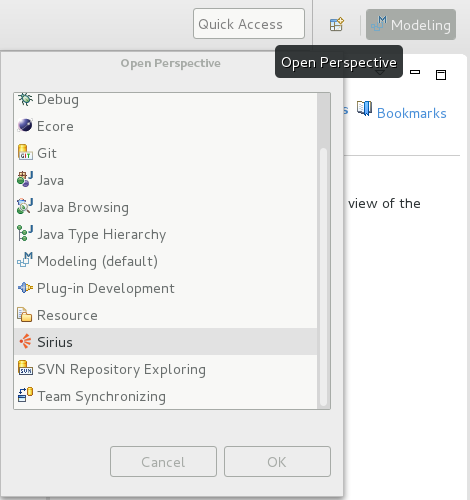
\includegraphics[width=8cm]{draws/sirius-persp.png}
 %    \caption{Sirius perspective}
     \label{fig:sirius-persp}
     }
% \end{figure}
\item
Create a new VCE project: right-click in the Model Explorer and select \textbf{New$\rightarrow$ Other...} (see a figure below). Then, select \textbf{VCE Wizard$\rightarrow$ VCE Project} and hit \textbf{Next}.
 %\begin{figure}
    \centerline{
     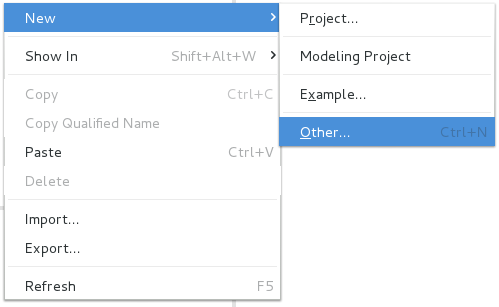
\includegraphics[width=7cm]{draws/new-other.png}
  %   \caption{New project creation}
     \label{fig:new-other}
     }
 %\end{figure}
 %\begin{figure}
     \centerline{
     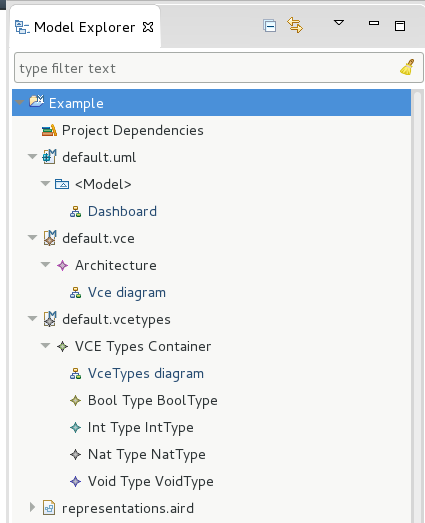
\includegraphics[width=7cm]{draws/vce-proj.png}
  %   \caption{VCE Wizard}
     \label{fig:vce-proj}
     }
 %\end{figure}
\item
Give a name to the project and press on \textbf{Finish};
\item
Right-click on the created project in Model explorer and select \textbf{Viewpoint selection}.
\item
Check all the viewpoints and press Ok.

     \centerline{
     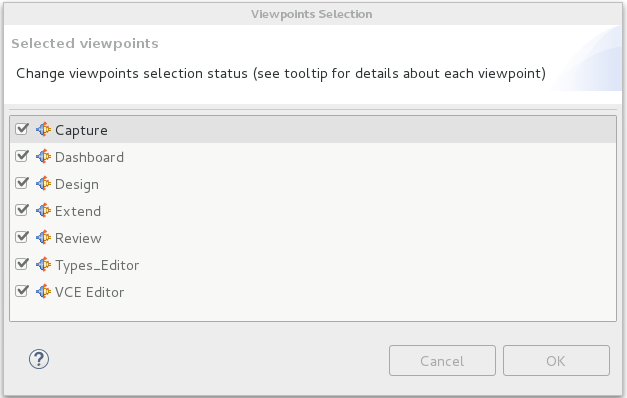
\includegraphics[width=11cm]{draws/viewpoints.png}
     %\caption{Viewpoints selection}
     \label{fig:viewpoints}
     }

\end{enumerate}

As a result, a new VCE project is created. Its structure is illustrated at the figure below.
 %\begin{figure}
     \centerline{
     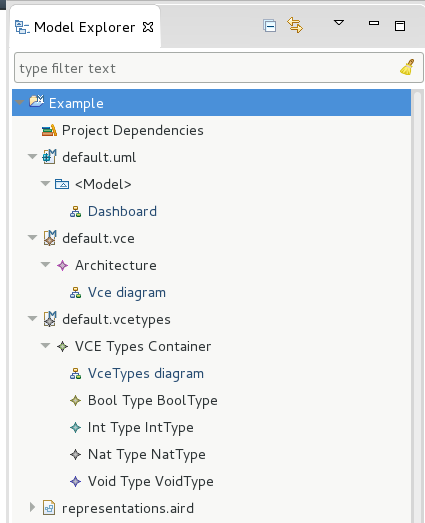
\includegraphics[width=10cm]{draws/vce-proj.png}
    % \caption{VCE Project Structure}
     \label{fig:vce-proj}
     }
 %\end{figure}
A VCE project has the following elements:
\begin{itemize}
\item
default.uml – a UML model;
\item
Dashboard - can be used to create diagrams;
\item
default.vce – a VCE model;
\item
VCE diagram - a diagram illustrating elements of default.vce;
\item
default.vcetypes – a model containing the types specification;
\item
VceTypes diagram - a diagram illustrating elements of default.vcetypes.
\end{itemize}

\subsection{Using an existing VCE Project }
When working in collaborative environments, you will often have to share projects with your colleagues. You may also have to download an existing project, usually in the form of an archive file, from existing sources. Importing such a project in your VCE workspace works as for any other Eclipse project:
\begin{enumerate}
\item
import the archive file (e.g. zip file), and save it somewhere on your file system;
\item
from the \textbf{File} menu, select \textbf{Import};
\item
select \textbf{General $\rightarrow$ Existing project in workspace} then hit Next;
\item
in the \textbf{Select archive file} item, Browse to find your archive file, hit Open;
\item
then hit Finish.
\end{enumerate}

The corresponding project will appear in the Model explorer panel, with a structure similar to the structure created by the VCE wizard, though of course there will usually many be more elements in there.

\subsection{Building the component Architecture in VCE component diagrams}\label{sec:comp-diagr}
This section describes how to edit model in VCE components diagrams.
\begin{enumerate}
\item
Normally, Components diagram should be created in a VCE project by default. In order to create a new diagram right-click on \textbf{Architecture} and chose \textbf{New Representation $\rightarrow$ new Components Diagram}.
\item
You can edit it using tools on the Palette. You can also use a toolbar on the top of a diagram editor. You can change the properties of your model elements using Properties View.
\end{enumerate}

For our first example pick-up the tool called \textbf{Primitive} and draw a primitive component. Then, add to the component two interfaces using \textbf{Server} and \textbf{Client} tools. You can edit the names either directly on the diagram of in the Properties view. The resulting diagram is illustrated at the figure below.

     \centerline{
     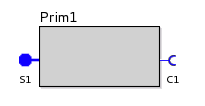
\includegraphics[width=6cm]{draws/prim.png}
    % \caption{VCE Project Structure}
     \label{fig:vce-proj}
     }
\subsection{Types specification}
This section describes how to specify the types. VCE has 4 predefined type: VoidType, BoolType, IntType and NatType. However, one can construct its own types: Enumerations, Records and specify integer intervals to abstract the data domains. Our example has one two integer intervals: \textbf{argType = 0..2} and \textbf{resType = 0..4}.

In order to specify the types, you need to:

\begin{enumerate}
\item
Open an existing VceTypes diagram or create a new one. In order to create a new diagram right-click on \textbf{VCE Types Container} in Model explorer and chose \textbf{new Representation $\rightarrow$ new Types Diagram}.
\item
You can edit it using tools on the Palette. 
\end{enumerate}

\textbf{Note: }in the current version of VCE most of the types features can be edited in \textbf{Properties} view but not directly.

For our first example pick-up the tool called \textbf{Intervals Container} and draw a a container where you will specify the intervals. Then, using \textbf{Int Interval} tool add two intervals. Use Properties view to set their names, lower and upper bounds. The result is illustrated below.

     \centerline{
     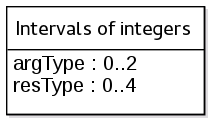
\includegraphics[width=4cm]{draws/types.png}
    % \caption{VCE Project Structure}
     \label{fig:vce-proj}
     }

\subsection{UML Classes and Interfaces}\label{sec:uml-classes}
The UML Classes, Interfaces and Operations that will be used to specify the GCM interfaces and the primitive component implementation class must be described at UML Class diagram. In order to create it, right-click on \textbf{$<$Model$>$} in the Model explorer and select \textbf{New Representation $\rightarrow$ Class diagram}. The new diagram will be created and opened automatically. Another way is to doube-click on \textbf{Dashboard} and there one can find Class diagram. 

[Hint]: choose meaningful, but reasonably short names. Long names make graphical diagrams difficult to manage] 

A figure below illustrates Class diagram of our example. 

     \centerline{
     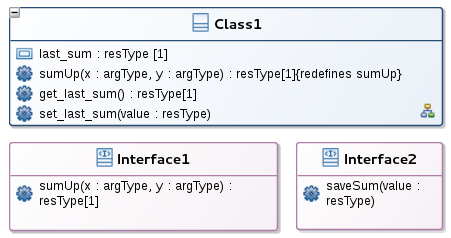
\includegraphics[width=12cm]{draws/classes.png}
    % \caption{VCE Project Structure}
     \label{fig:vce-proj}
     }

It has two UML Interfaces: \textbf{Interface1} and \textbf{Interface2}, and one UML Class \textbf{Class1}. In order to create them, \textbf{Interface} (resp. \textbf{Class}) tools are used.
The tool \textbf{Operation} is used in order to add an Operation to a Class or an Interface (pick-up the tool and click on the Class or Interface where you want to add the Operation). You can modify the Operation in its Properties view. The name can be set in \textbf{General} tab.  The specification of the arguments and return type is a little bit more tricky. In order to modify them, you need to:

\begin{enumerate}
\item
Go to the Parameters tab of the Operation Properties view.
\item
Click on the \textbf{green plus} button in the top-right corner of the Properties view; this will open a window to create a parameter as illustrated on the figure below.

     \centerline{
     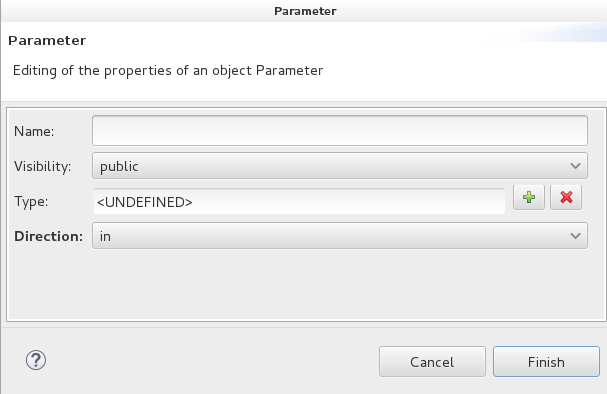
\includegraphics[width=10cm]{draws/param-empty.png}
    % \caption{VCE Project Structure}
     \label{fig:vce-proj}
     }
     
\item
The window includes fields for specification of the name, type and direction of the parameter. You parameter can be either an argument of an operation, or its return type. Enter the name if you are specifying an argument; select the direction: \textit{in} for the arguments or \textit{return} for the return type. You should also select the parameter type among the ones declared in the VceTypes model. In order to specify the type, click on \textbf{green plus} button next to the field Type, go to \textbf{All Resources} tab and select the needed VceType from your .vcetypes model. See an example below.

     \centerline{
     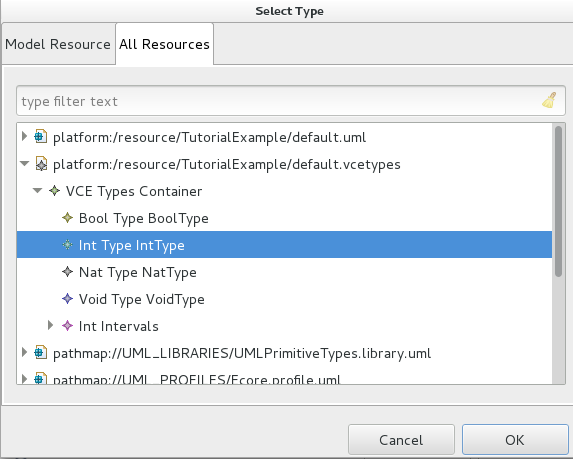
\includegraphics[width=11cm]{draws/param-type.png}
    % \caption{VCE Project Structure}
     \label{fig:vce-proj}
     }

The example of \textbf{x} argument of \textbf{sumUp} operation is given on the figure below.

     \centerline{
     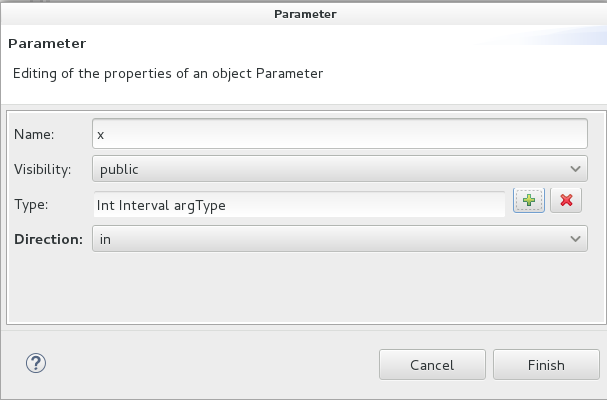
\includegraphics[width=12cm]{draws/param.png}
    % \caption{VCE Project Structure}
     \label{fig:vce-proj}
     }

\end{enumerate}

An attribute (or  property) of a class can be specified using a tool \textbf{Property}. Among the properties of an attribute the most important ones are its name, type and default value.

\subsection{Types of UML Class Operations}
We should distinguish three types of UML Class Operations:
\begin{itemize}
\item
\textbf{Server operations}. These are the operations that will be accessed from outside of a component. They implement the behavior of server interfaces operations. In order to establish the relation between a server operation of a class and the implemented method of an interface you need to do the following. (1) go to the Properties view of your class operation and open \textbf{Semantic} tab. (2) in the field \textbf{Redefined operation} select the implemented operation of an interface.
\item
\textbf{Local operations}. These are class operations that are used for local computations and are not accessible from outside of the component.
\item
\textbf{Get and set operations}. This is a special kind of local operations that are used inside the component to get or set the value of its attributes. One get and one set operation should be manually declared for \textit{every attribute of a Class}. The signature of a get operation is \textsf{get\_attrName():attrType}; the signature of a set operation is \textsf{set\_attrName(value:attrType)}.
\end{itemize}

\subsection{Attach a UML Interface to a GCM Interface}
In our example, a UML Interface S1 is attached to a GCM Interface Interface1 and Interface2 is attached to C1. Which means that operations of Interface1 can be called on S1 and operations of Interface2 can be called from C1. In order to attach a UML Interface to a GCM Interface you need to:
\begin{enumerate}
\item
Open the VCE Components Diagram.
\item
Right-click on the GCM interface to which you want to attach a UML Interface (S1 or C1 in our example).
\item
Select \textit{Attach UML Interface} option.
\item
Select the required UML interface from the given list (Interface1 of Interface2 in our example)
\end{enumerate}

In the case of our example if you specify everything correctly, you should get the diagram illustrated below.

     \centerline{
     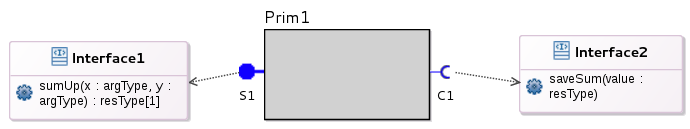
\includegraphics[width=14cm]{draws/itfs.png}
    % \caption{VCE Project Structure}
     \label{fig:vce-proj}
     }
     
\subsection{Attach a UML Class to a GCM Component}
UML classes illustrate the lists of the operations that can be processed by the GCM primitive components and the list of possessed attributes. In our example, Class1 contains the methods of a component Prim1. In order to specify the relation between a primitive and its implementation class, right-click on the primitive component and select \textit{Attach UML Class} option. Then, select the required class from the given list. The result is illustrated on the figure below.

     \centerline{
     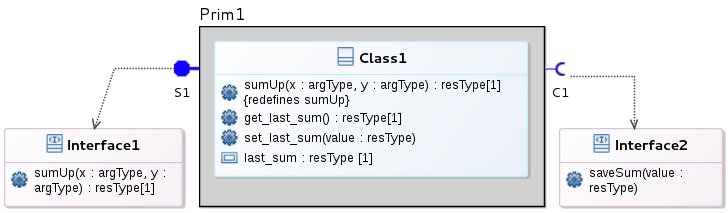
\includegraphics[width=14cm]{draws/prim-class.png}
    % \caption{VCE Project Structure}
     \label{fig:vce-proj}
     }

\subsection{Component attributes}
A UML class attached to a primitive component defines the list of the component's attributes. The default value of an attribute can be always set on the UML Class Diagram. However, it is often needed to set the default value of an attribute in the context of a a concrete primitive component. In order to do so you should:

\begin{enumerate}
\item
Open VCE Components Diagram.
\item 
Pick-up \textbf{Attributes specification} tool and add a box for attributes specification to the primitive component.
\item
Use tool \textbf{Attribute value} to add attributes that have specific default value to the attributes specification box. 
\item
You can set the name and the value of an attribute in Properties view. \textbf{Note:} the name of the attribute should strictly correspond to the one on a Class diagram.
\end{enumerate}

The example of the resulting diagram is given on the figure below.

     \centerline{
     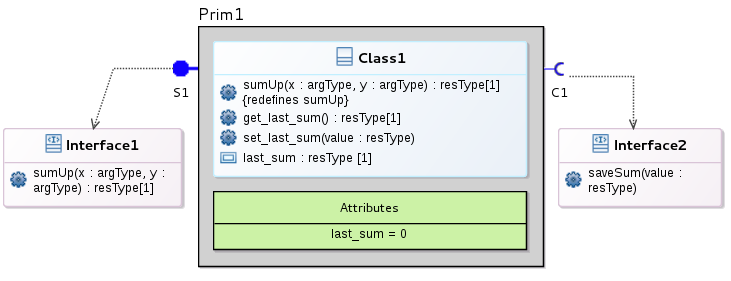
\includegraphics[width=14cm]{draws/prim-attr.png}
    % \caption{VCE Project Structure}
     \label{fig:vce-proj}
     }
     
\subsection{Create and attach a State Machine to a UML Operation}

State Machines define the behavior of operations of UML classes. In order to specify a State Machine of an operation you need to:

\begin{enumerate}
\item
Open a .uml file (UML model) in a standard EMF editor and go to the UML Class which operation behavior you want to specify. Right-click on the class and select \textbf{New Child $\rightarrow$ Classifier Behavior $\rightarrow$ State Machine}. This will create an instance of the State Machine. You can specify its name in the Properties view. An example is given below.

     \centerline{
     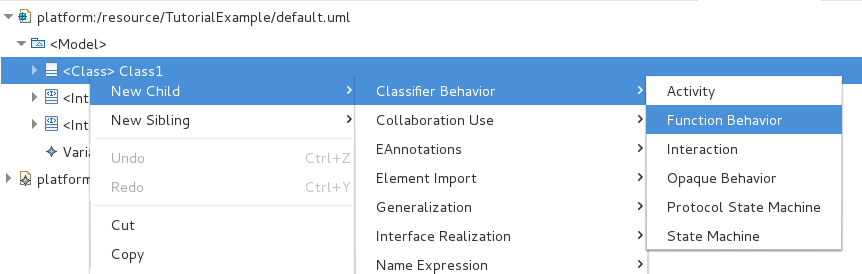
\includegraphics[width=14cm]{draws/sm-creation.png}
    % \caption{VCE Project Structure}
     \label{fig:vce-proj}
     }

\item 
Add a region to the State Machine in a similar way.
\item
Save the model. Now you can create a diagram of your State Machine.
\item
Right-click on the created State Machine in Model Explorer and select \textbf{New Representation $\rightarrow$ State Machine diagram}. Specify the name of the diagram and hit Ok.

     \centerline{
     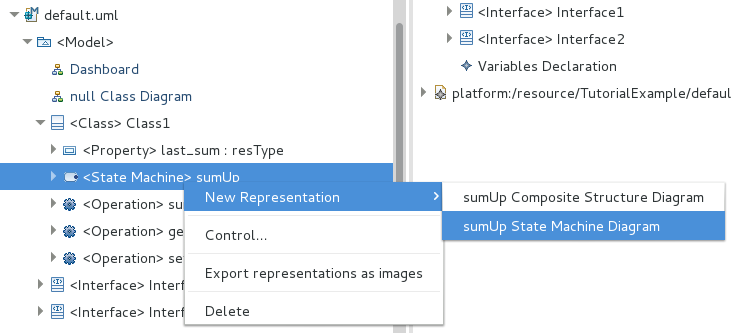
\includegraphics[width=10cm]{draws/sm-diagr.png}
    % \caption{VCE Project Structure}
     \label{fig:vce-proj}
     }
\end{enumerate}

\textbf{Note! }Set/get methods should NOT have State Machines attached. Their implementation is default in the current version of VerCors.

\subsection{Edit the Local variables of a State Machine }
If you want to use local variables on your State Machine, you should declare them in a specific section on a State Machine Diagram called \textbf{Local variables}. You should add one box for the local variables declaration to you state machine diagram using a tool \textbf{VDCreation}. Then, you can add local variables to the box using \textbf{Variable} tool. You should set the names and types of variables in the Properties view. Figure below illustrates local variables of our example.

     \centerline{
     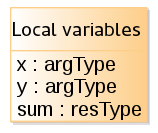
\includegraphics[width=3cm]{draws/loc-var.png}
    % \caption{VCE Project Structure}
     \label{fig:vce-proj}
     }
     
\subsection{Edit State Machines}
You can use Palette of the State Machine Diagrams to add transitions and states. You can also directly edit labels of states and transitions. To follow our example you can first add states and transitions to your State Machine Diagram as illustrated below.

     \centerline{
     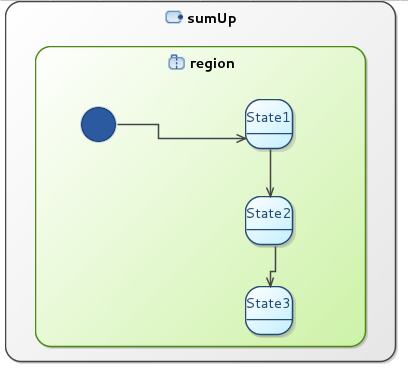
\includegraphics[width=5cm]{draws/sm-no-lbl.png}
    % \caption{VCE Project Structure}
     \label{fig:vce-proj}
     }
     
The behavior of the methods if specified on the state machines transitions labels. In order to edit a label you need click on it once in order to select it. Then, you can click on it second time to edit it. From a state machine you have access to the local methods of the class owning the state machine , to the methods of client interfaces and to the local variables of the state machine. The attributes of the class. The labels text should correspond to the grammar given below.

\begin{grammar}

<Transition_label> ::= '[' <Guard_Expr> ']' \alt '/' <Stms> \alt  '['<Guard_Expr>']'\alt '/' <Stms>

<Stms> ::= <Stm> ';' \alt <Stm> ';' <Stms> \alt <MCall> \alt <Return>

<Stm> ::= <Assign> 

<Assign> ::= <Variable> ':='  <Expr> \alt <Variable> ':=' <MCall>

<Expr> ::=  <Variable> \alt <Constant> \alt  <Expr> <Bop> <Expr> \alt '('<Expr>')'

<MCall> ::= ID'.'ID '( )' \alt 
	 ID'.'ID '(' <Args> ')' \alt 
	 'this.'ID '( )' \alt 
	'this.'ID  '(' <Args> ')'
	 
<Args> ::=  <Constant> \alt> <Variable> \alt <Args> ',' <Args>

<Constant> ::= NUM \alt <Boolean_constant>

<Bop> ::=  '\&\&' \alt  '||'  \alt '+' \alt '-' \alt '*' \alt '/' \alt '=' \alt '$>$=' \alt '$>$' \alt '\textless'  \alt '\textless='

<Boolean_constant> ::= 'true' \alt 'false'

<Guard_Expr> ::= <Expr>

<Return> ::= 'return' <Variable> \alt 'return' <Constant> \alt  'return'

\end{grammar}

The final version of sumUp state machine of our example is given on the figure below.

     \centerline{
     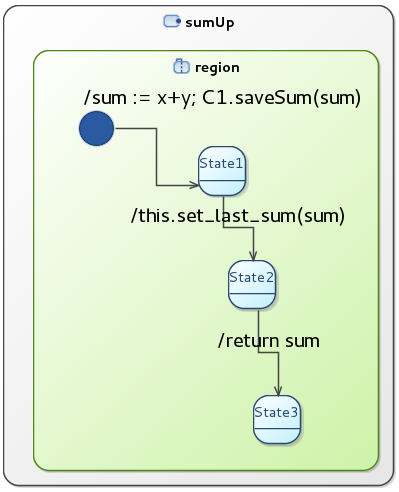
\includegraphics[width=7cm]{draws/sm.png}
    % \caption{VCE Project Structure}
     \label{fig:vce-proj}
     }

\section{Diagram Validation}
Before using the diagrams, and in particular before generating ADL files, it is mandatory to check the structural coherency of the semantics. In order to do this open a VCE Components Diagram and select \textbf{Diagram $\rightarrow$ Validate} in the menu. 

The elements of the diagram which did not pass the validation should be marked with red signs. You will also see the validation errors/warnings description in the Problems view, and in the Model explorer.

A figure below illustrates an example of a non-valid model. The interfaces of Composite1 did not pass the validation because they have the same names. The binding did not pass the validation because it goes from a server interface to a server interface.

     \centerline{
     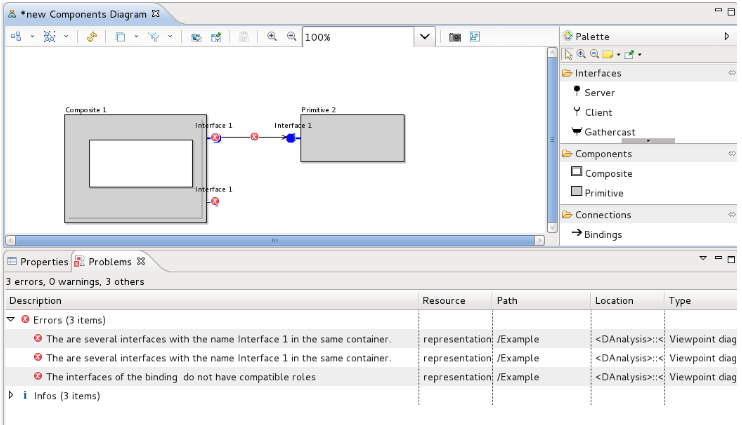
\includegraphics[width=14cm]{draws/valid.png}
    % \caption{VCE Project Structure}
     \label{fig:vce-proj}
     }

The violation of the following constraints are considered to be an error:
\begin{itemize}
\item
Bindings do not cross a component border;
\item
The interfaces connected by a binding have compatible types;
\item
The interfaces connected by a binding have compatible roles;
\item
The interfaces connected by a binding have compatible natures;
\item
All the interfaces in the same container have different names;
\item
All the components in the same container have different names;
\item
The violation of the following constraints are considered to be a warning:
\item
The interfaces connected with a binding should have different containers;
\item
The violation of the following constraints are considered to have the information level:
\item
Each GCM interface should have a reference to a UML interface.
\end{itemize}

\subsection{Generating executable GCM/ProActive files}
Once a component diagram has been checked valid, it is possible to generate automatically some of the files necessary for building a GCM/ProActive executable application. More precisely the generated files are:
\begin{itemize}
\item
one ADL file, in XML format respecting the ADL DTD "classpath://org/objectweb/proactive/core/component/adl/xml/proactive.dtd". It represents the application component architecture (components, interfaces, bindings), and the link with the interface and content Java classes;
\item
one Java interface file for each UML interface in the application;
\item
one Java class per UML class specified on Class diagram;
\item
one Java interface for every UML class attached to a primitive component with attributes specification (such component becomes an attribute controller in terms of GCM/ProActive and needs an interface to be implemented);
\item
one Java class per each Enumeration and Record type from the VceTypes model;
\item
a Java enumeration State used for methods implementation
\end{itemize}

VerCors partially generates executable code of class operations. For those operations that have State Machines attached it translate State Machines into Java code. It also generates the code of set/get methods to access attributes of the Java classes.

\section{Generation of input for CADP}

The graphically specified models are translated by VerCors into low-level models encoding the behavior of a GCM applications. PNets and pLTS are used to encode the behavior as described here\footnote{https://hal.inria.fr/hal-00761073}.

In order to assist model-checking of the specified models, VerCors generates the following files:
\begin{itemize}
\item
a .fcr file per each pLTS;
\item
a .exp file per each pNet;
\item
.svl script that optimizes models and calls script transforming .exp files into .bcg
\item
run.sh script that calls .svl scripts and flac-and-minimize script on all .fcr files.
\end{itemize}

\textbf{Note! } The current version of VerCors generates data only from a composite that contains several primitives in its content. Membrane, group interfaces, non-functional interfaces and composite components inside a content are not supported in the current version.

To generate a pNet of a composite you need to:
\begin{enumerate}
\item
Right-click on the representation of the Composite component on VCE Components Diagram and select \textbf{Generate pNet $\rightarrow$ Generate pNet}. This will open the wizard where you can step-by-step specify the parameters of the verified system.
\item
Select the State Machine of the environment scenario.
\item
Specify the queue size of the root component as well as its sub-components.
\item
Specify the communications that you do not want to observe during the model-checking.
\end{enumerate}

\textbf{Node! } In current version does not perform any type-checking of your model.

\end{document}